% --------------------------------------------------------------------------------
% ---------------------------------  Preamble  -----------------------------------
% --------------------------------------------------------------------------------

\documentclass{article}

\usepackage[defaultfam,tabular]{montserrat}
\usepackage[letterpaper, margin=0.75in]{geometry}
\usepackage{graphicx}               % to insert figures
\usepackage[table,x11names]{xcolor} % colors for e-copies
\usepackage{subcaption}             % subfigures
\usepackage{placeins}               % Float barriers
\usepackage{booktabs}
\usepackage{array}
\usepackage{caption}
\usepackage{rotating}
\usepackage{multicol}
\usepackage{multirow}
\usepackage{titlesec}
\usepackage{hyperref}               % PDF hyperreferences
\usepackage{titling}
\usepackage{tikz}
\usetikzlibrary{shapes.geometric}
\usetikzlibrary{calc}
\usepackage[T1]{fontenc}
\renewcommand*\oldstylenums[1]{{\fontfamily{Montserrat-TOsF}\selectfont #1}}

\newsavebox{\savefig}

\setcounter{secnumdepth}{0}

\titleformat{\section}[block]
  {\normalfont\fontsize{16}{17}\fontseries{ub}\selectfont}
  {\thesection\enspace}{0pt}{\centering\MakeUppercase}[\vspace{2pt}{\titlerule[2pt]}]

\titleformat{\subsection}[block]
  {\titlerule\addvspace{3pt}\bfseries\centering}
  {\thesection\enspace}{0pt}{\MakeUppercase}[\vspace{3pt}\titlerule]

\titleformat{\subsubsection} [block]{\bfseries}{}{0em}{\MakeUppercase}

\renewcommand\maketitlehooka{\null\mbox{}\vfill}
\renewcommand\maketitlehookd{\vfill\null}
\title{
  \fontfamily{Montserrat-TOsF}\selectfont
  \fontsize{50}{60}\fontseries{ub}\selectfont\textcolor{white}{\MakeUppercase{B}}
\includegraphics[width=0.5in]{../img/Battletech_A.png}\fontsize{50}{60}\fontseries{ub}\selectfont\textcolor{white}{\MakeUppercase{ttleTech}}\\
  \fontsize{35}{42}\fontseries{ub}\selectfont\MakeUppercase{Outworlds Wastes}\\
  ~\\
  
\includegraphics[width=4in]{../img/Outworlds_Alliance.png}
  ~\\
  ~\\
  \LARGE\bfseries{Casual BattleTech League Framework} \\
}
\author{}
\date{}

% Optional PDF information
\ifpdf
\hypersetup{
  pdftitle={Outworlds Wastes},
  pdfauthor={Jeremy L Thompson}
}
\fi

\setlength\parskip{5pt plus 2pt minus 1pt}

% --------------------------------------------------------------------------------
% ---------------------------------  Document  -----------------------------------
% --------------------------------------------------------------------------------

\begin{document}

\clearpage

% --------------------------------------------------------------------------------
\maketitle
% --------------------------------------------------------------------------------

\AddToHookNext{shipout/background}
{\put(0,-\paperheight)
  {%
   
\begin{tikzpicture}
   \fill[use as bounding box,black!10] (current page.north west) rectangle (\paperwidth,0);
   \fill[use as bounding box,black!50] ($ (current page.north west)+(0,-5.35) $) rectangle ++(\paperwidth,-1.7);
   \fill[use as bounding box,black!30] ($ (current page.north west)+(0,-7.05) $) rectangle ++(\paperwidth,-1.6);
   \fill[use as bounding box,black!30] ($ (current page.north west)+(0,-21.5) $) rectangle ++(\paperwidth,-0.9);
   \end{tikzpicture}
  }
}

\thispagestyle{empty}

\newpage

% --------------------------------------------------------------------------------
% --------------------------------------------------------------------------------
\section{BattleTech: Outworlds Wastes}
% --------------------------------------------------------------------------------
% --------------------------------------------------------------------------------

\emph{BattleTech: Outworlds Wastes} is a casual BattleTech league framework with simplified logistics rules.
Players will take the role of commander of a mech force searching the Outworlds Wastes for lost technology and glory.
Completing objectives in scenarios will earn C-bills that commanders can use to upgrade their forces.
Different formats of scenario play are supported, to include Classic BattleTech, Alpha Strike, and BattleTech: Override.

% --------------------------------------------------------------------------------
\subsubsection*{Goals}
% --------------------------------------------------------------------------------

\begin{itemize}

\item Have lots of fun while fostering a friendly and welcoming environment.

\item Give players an opportunity to build personalized lore for their own BattleTech forces.

\item Provide a lightweight framework for players to track the accomplishments of their forces.

\item Explore BattleTech lore and equipment.

\item Require minimal resources beyond \emph{BattleTech: Total Warfare} and the \emph{Master Unit List}.

\item Support players across a variety of experience levels.

\end{itemize}

% --------------------------------------------------------------------------------
\subsubsection*{Contents}
% --------------------------------------------------------------------------------

These rules cover four general areas: background information, player information, league organizer information, and reference material.
Background information describes the Outworlds Wastes region and the overall design of the Outworlds Wastes league.
Force Construction rules, page \pageref{subsec:force_construction}, and Force Maintenance and Improvements rules, page \pageref{subsec:force_maintenance}, are the minimum rules needed for a player to jump into Outworlds Wastes league play.
Scenario design and league scoring rules are provided for league organizers.
The remaining content is reference material, to include a region map and sample tables for tracking a player's forces.

% --------------------------------------------------------------------------------
\subsubsection*{Disclaimer}
% --------------------------------------------------------------------------------

This rule system is fan-made, based upon official BattleTech rules from Catalyst Game Labs, and only adds simplified campaign logistics and force management rules.
See the \emph{References} section for a list of official Catalyst Game Labs products that \emph{BattleTech: Outworlds Wastes} specifically references.

% --------------------------------------------------------------------------------
\subsubsection*{Version}
% --------------------------------------------------------------------------------

This document is current as of \today.

\newpage

% --------------------------------------------------------------------------------
% --------------------------------------------------------------------------------
\tableofcontents
% --------------------------------------------------------------------------------
% --------------------------------------------------------------------------------

\newpage

% --------------------------------------------------------------------------------
% --------------------------------------------------------------------------------
\section{Background}
% --------------------------------------------------------------------------------
% --------------------------------------------------------------------------------

The Outworlds Alliance was founded in 2413 and enjoyed prosperity throughout the Star League Era.
By the start of the Amaris Civil War in 2766, the Outworlds Alliance contained over 135 major systems across 7 administrative districts.
Unfortunately, the Outworlds Alliance suffered during the Succession Wars that followed the fall of the Star League in 2780, and they had to steadily abandon systems that they no longer had the resources to support.

Clan Snow Raven began exploring the Periphery for resources soon after the battle of Tukayyid ended Operation REVIVAL.
In 3064, Clan Snow Raven and the Outworlds Alliance began developing mutual respect and tentative alliance.
Following their abjuration from the Clan Homeworlds in 3075 as a result of the Wars of Reaving, Clan Snow Raven took refuge in the Outworlds Alliance.
In 3083, Clan Snow Raven and the Outworlds Alliance merged to form the Raven Alliance.
By the ilClan Trial in 3151, the Raven Alliance contained only 47 systems.

The exact number of systems varies from era to era, but approximately 88 systems that were part of the Outworlds Alliance during the Star League era have been lost.
These lost worlds form the Outworlds Wastes.
Many factions are eager to explore these lost worlds in the Outworlds Wastes in search of lost Star League technology or to take refuge from the complex political machinations of the Inner Sphere.

You will take the role of commander of a mech force exploring the Outworlds Wastes for your faction during the current league era.
Common factions for the region include

\begin{multicols}{2}

\begin{itemize}

\item Outworlds Alliance

\item Clan Snow Raven

\item Draconis Combine

\item Federated Suns

\item Mercenary groups

\item Pirate gangs

\item Clan Dark Caste\\~\\

\end{itemize}

\end{multicols}

Commanders should pick the faction they are most interested in representing.
While the major factions are the most prevalent in the region, other factions may be found in the Outworlds Wastes.
For example, the Raven Alliance has relationships with nations on the far side of the Periphery, such as Magistracy of Canopus.

Commanders will compete with other factions in the Outworlds Wastes to grow their force and recover lost technology.
Scenarios are primarily designed for Classic BattleTech, but scenarios for Alpha Strike and BattleTech: Override is also supported.

League organizers pick the era for the current league; organizers can select any era after the fall of the Star League.
The era determines unit availability and the most common factions in the Outworlds Wastes.
Commanders should ask the league organizer which era is being used.

\newpage

% --------------------------------------------------------------------------------
% --------------------------------------------------------------------------------
\section{Force Management}
% --------------------------------------------------------------------------------
% --------------------------------------------------------------------------------

Unit commanders start with 10,000 Battle Value points (BV) they can use to purchase their initial units and 3,000,000 C-bills they can use after completing the first mission.
Completing scenarios and accomplishing objectives will earn additional C-bills for commanders to spend on training their pilots, upgrading units, and acquiring new equipment.

% --------------------------------------------------------------------------------
\subsection{Force Construction}
\label{subsec:force_construction}
% --------------------------------------------------------------------------------

Commanders start with 10,000 BV to acquire initial units for their force.
BV costs for all units are listed in the \href{http://www.masterunitlist.info}{Master Unit List} or \href{https://megamek.org}{MegaMekLab}.
Force construction must follow these rules:

\begin{itemize}

\item Commanders have a modified Union class dropship with 16 configurable bays.
Each bay can hold 1 mech, 2 combat vehicles, 2 aerospace units, 5 protomechs, 1 mechanized infantry unit, or 5 tons of battle armor/non-mechanized infantry.
Bay space for all xattle armor and non-mechanized infantry units is shared; for example, 4 bays can hold 20 tons, which is 5 squads of inner sphere standard battle armor.
The dropship may have no more than 12 mech bays, 5 combat vehicle bays, 2 aerospace bays, 2 protomech bays, or 5 infantry/battle armor bays.
Bays can be empty or changed between configurations.
Your entire force must fit onto your dropship.

\item Commanders should select units from their faction on the \href{http://www.masterunitlist.info/}{Master Unit List} for the era chosen by league organizers.
Forces can include units with introductory, standard, and advanced technology.
For example, the Marauder MAD-3R, Marauder MAD-7R, and Marauder II MAD-6C are legal ilClan era mercenary units while the Marauder II MAD-6M is not.
Forces can include one unique or experimental unit.

\item Each force can start with no more than 7,000 BV in mechs.
Commanders are encouraged to try to use the typical mech unit composition of their faction.
However, this can be difficult to accomplish for clan or ComStar forces, so this is not a requirement.

\item Each force can include any number of supporting units, such as combat vehicles, protomechs, battle armor, and infantry, so long as the dropship bay restrictions are met.
Some scenarios will require infantry or battle armor and combat vehicles with cargo capacity, so commanders should have at least one of each of these units in their force.

\item Forces cannot contain off-map battlefield support units, such as artillery or aerospace fighters.
However, forces can contain any on-map units.

\item The BV costs of a unit includes the skill levels.
Skill levels should generally be close to the average skill levels given on page 40 of \emph{BattleTech: Total Warfare}.
The skill levels for a unit may be no better than Gunnery 3/Piloting 4.

\end{itemize}

One of the goals of the Outworlds Wastes framework is to explore different equipment.
Commanders are encouraged to know where in the rule books other commanders can read about the rules pertaining to any special equipment for units in their force.
Unit record sheets for units can be generated using \href{https://megamek.org}{MegaMekLab} or similar tools.

Learning new types of units can be intimidating, especially in Classic BattleTech.
Commanders are welcome to limit the number of types of units in their non-mech forces.
For example, a force could include only troop transports and battle armor so the commander can meet any objective while keeping new rules to a minimum.

\newpage

Two sample initial forces are provided; the first force is a Civil War era mercenary company and the second force is an ilClan era Raven Alliance nova.
Mech pilot names are encouraged, as one of the goals is to develop the personalized lore for your force.

\begin{table}[h!]
\fontfamily{Montserrat-LF}\selectfont
\centering
\newcolumntype{R}[1]{>{\raggedleft\let\newline\\\arraybackslash\hspace{0pt}}m{#1}}
\begin{tabular}{| m{1.5em} m{12em} m{8em} R{4.6em} R{4.6em} R{3.5em} R{3.8em} |}
\hline
\rowcolor{black!30}  \bfseries{Bay} & \bfseries{Unit} & \bfseries{Pilot} & \bfseries{Gunnery} & \bfseries{Piloting} & \bfseries{BV} & \bfseries{Adj BV} \\
\hline
\rowcolor{black!30} \multicolumn{7}{|c|}{Mechs} \\
\hline
1   & Atlas II AS7-D        & 'Meg' Courant    & 3       & 4         & 1,897 & 2,504 \\
2   & Phoenix Hawk PXH-2K   & 'Bison' Helge    & 4       & 5         & 1,271 & 1,271 \\
3   & Blackjack BJ-2        & 'Lizard' Baker   & 4       & 5         & 1,148 & 1,148 \\
4   & Locust IIC            & 'Casper' Poole   & 4       & 5         & 1,100 & 1,100 \\
\hline
\rowcolor{black!30}\multicolumn{7}{|c|}{Combat Vehicles} \\
\hline
1  & Maxim Hover Transport &                   & 4       & 5         &   764 &   764 \\
1  & Maxim Hover Transport &                   & 4       & 5         &   764 &   764 \\
2  & Galleon GAL-102       &                   & 4       & 5         &   651 &   651 \\
2  & Galleon GAL-102       &                   & 4       & 5         &   651 &   651 \\
3  & Warrior H-7           &                   & 4       & 5         &   295 &   295 \\
3  & Warrior H-7           &                   & 4       & 5         &   295 &   295 \\
\hline
\rowcolor{black!30}\multicolumn{7}{|c|}{Infantry/Battle Armor} \\
\hline
1  & IS Std BA, LRR        &                   & 4       & 5         &   255 &   255 \\
2  & IS Std BA, Laser      &                   & 4       & 5         &   231 &   231 \\
\hline
9  & Total Bays            &                   &         &           &       &       \\
   & Total BV              &                   &         &           &       & 9,929 \\
\bottomrule
\end{tabular}
\caption*{Civil War Era Mercenary Force - Meg's Magpies}
\end{table}

\begin{table}[h!]
\fontfamily{Montserrat-LF}\selectfont
\centering
\newcolumntype{R}[1]{>{\raggedleft\let\newline\\\arraybackslash\hspace{0pt}}m{#1}}
\begin{tabular}{| m{1.5em} m{12em} m{8em} R{4.6em} R{4.6em} R{3.5em} R{3.8em} |}
\hline
\rowcolor{black!30}  \bfseries{Bay} & \bfseries{Unit} & \bfseries{Pilot} & \bfseries{Gunnery} & \bfseries{Piloting} & \bfseries{BV} & \bfseries{Adj BV} \\
\hline
\rowcolor{black!30}\multicolumn{7}{|c|}{Mechs} \\
\hline
1   & Carrion Crow A        & Sarah Magnus    & 3       & 4         & 1,622 & 2,141 \\
2   & Nova U                &       Bryn      & 4       & 5         & 1,413 & 1,413 \\
3   & Adder J               &       Ada       & 4       & 5         & 1,222 & 1,222 \\
4   & Kit Fox V             &       Soton     & 3       & 4         &   974 & 1,286 \\
5   & Fire Moth A           &       Tina      & 3       & 4         &   639 &   843 \\
\hline
\rowcolor{black!30}\multicolumn{7}{|c|}{Combat Vehicles} \\
\hline
1   & Karnov UR Transport   &                 & 4       & 5          &   125 &   125 \\
\hline
\rowcolor{black!30}\multicolumn{7}{|c|}{Infantry/Battle Armor} \\
\hline
1   & Gnome BA              &                 & 3       & 4         &   580 &   766 \\
2   & Elemental BA, Laser   &                 & 3       & 4         &   447 &   590 \\
3   & Elemental BA, HMG     &                 & 3       & 4         &   415 &   548 \\
4   & Elemental BA, Flamer  &                 & 3       & 4         &   404 &   533 \\
5   & Elemental BA, Flamer  &                 & 3       & 4         &   404 &   533 \\
\hline
11  & Total Bays            &                 &         &           &       &       \\
    & Total BV              &                 &         &           &       & 10,000 \\
\hline
\end{tabular}
\caption*{ilClan Era Raven Alliance Force - Raven Expeditionary Cluster, Alpha Nova}
\end{table}

Both forces can support additional units on their dropships.
However, the Raven Expeditionary Cluster, Alpha Nova force cannot support any additional infantry/battle armor bays because their dropship is using the maximum of 5 bays.

\newpage

% --------------------------------------------------------------------------------
\subsection{Advanced Force Construction Rules}
% --------------------------------------------------------------------------------

The \href{http://www.masterunitlist.info/}{Master Unit List} provides all factions from official BattleTech lore.
A commander can create a modified faction list representing their custom faction.

To create a custom faction list, go to the \href{http://www.masterunitlist.info/Unit/Filter}{Units Tab on Master Unit List}.
Filter the units to include one faction list and one general list.
For example, the Pirates faction by default typically includes the Periphery General list.
A Dark Caste custom faction might include the Pirates faction list with the Inner Sphere Clan General list.

Be sure to also filter by the appropriate Availability Era for the current league era.
All restrictions from the basic Force Construction rules, such as technology level and bay limits, still apply.

Any faction that has a general list can be modified with these rules.
If the faction does not have a general list, then it cannot be customized in this way.
Factions without a general list include Mercenary, Kell Hounds, Wolf's Dragoons, and Society.
These factions have the phrase "including Blank General List" on their faction and era specific page.
Adding a general list to these factions would give the commander a disproportionately large number of units to choose from.

Commanders can still create a custom mercenary faction with these Advanced Force Construction Rules.
First select a faction list for the region in which the force was founded or primarily operates and then pick an appropriate general list.
For example, a mercenary force that was founded in the Draconis Combine but moved to the Periphery after Coordinator Takashi Kurita's \emph{Death to Mercenaries} edict could use Draconis Combine faction list with the Periphery General list.

\begin{figure}[h!]
  \centering
  \begin{subfigure}{0.4\textwidth}
    \centering
    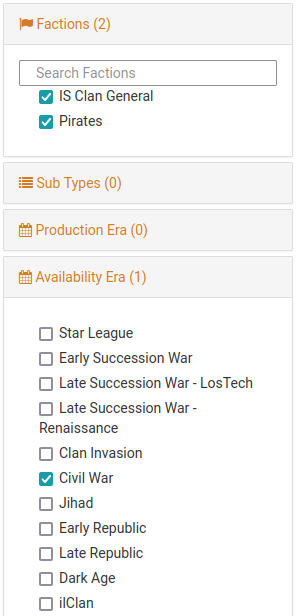
\includegraphics[height=5.0in]{../img/Dark_Caste_List.png}
    \caption*{Dark Caste Faction}
  \end{subfigure}
  \hspace{1in}
  \begin{subfigure}{0.4\textwidth}
    \centering
    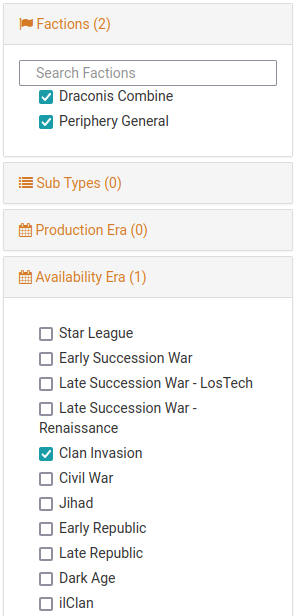
\includegraphics[height=5.0in]{../img/Combine_Mercenary_List.png}
    \caption*{Combine Mercenary Faction}
  \end{subfigure}
  \caption*{Custom Faction Lists}
\end{figure}

\newpage

% --------------------------------------------------------------------------------
\subsection{Force Maintenance and Improvements}
\label{subsec:force_maintenance}
% --------------------------------------------------------------------------------

Commanders can spend C-bills they earn in scenarios to improve their force.
Possible improvements are listed below.
C-bill costs for all units are listed on the \href{http://www.masterunitlist.info}{Master Unit List}.
The C-bill cost in \href{https://megamek.org}{MegaMekLab} can be used if the \href{http://www.masterunitlist.info}{Master Unit List} does not list a cost.

\begin{itemize}

\item {\bfseries Train}: Pay 500,000 C-bills multiplied by the difference in BV skill multiplier to improve a unit's skill levels.
For example, a Gunnery 4/Piloting 5 pilot has a BV skill multiplier of 1.0 and a 3/4 pilot has a BV skill multiplier of 1.32.
Therefore, it costs 160,000 C-bills to train a 4/5 pilot to be a 3/4 pilot.
All units cannot be upgraded past 1/2.
New pilots/crew cannot be upgraded past 3/4.
Old units that did not participate in the most recent scenario cannot be upgraded past 4/5.
See \emph{BattleTech: TechManual}, page 315, for the BV skill multiplier table.
A unit's skill levels can be degraded at no C-bill cost.

\item {\bfseries Replace}: Pay 50\% of the C-bill cost, rounded up, to replace a \emph{destroyed} unit.
If the mech pilot or vehicle crew was killed, the replacement cost includes a 5/6 pilot or crew.
If an entire infantry or battle armor unit was destroyed, the replacement cost includes 5/6 troops.
The protomech replacement cost includes a 5/6 pilot.
The new unit can be trained as above.
See \emph{BattleTech: Total Warfare} for the definition of \emph{destroyed} for different types of units.

\item {\bfseries Repair}: Pay 25\% of the C-bill cost, rounded up, to repair all internal damage and critical components for a unit that has not been \emph{destroyed}.
If the pilot or crew was killed, the repair cost includes a 5/6 pilot or crew.
Armor repairs have no C-bill cost.

\item {\bfseries Recruit}: Pay 50\% of the C-bill cost, rounded up, recruit new troops to replace troops in an infantry or battle armor unit that has not been \emph{destroyed}.
For example, if 1 out of 4 troops was killed in a battle armor squad, pay 50\% of the C-bill cost for 1 suit.
To replace 1 troop in a squad of 4 IS Standard Battle Armor with Lasers, pay 293,125 C-bills.
Damage to battle armor troops that survive a scenario is repaired for free.

\item {\bfseries Refit}: Pay the difference in C-bill cost to refit a unit to a different variant.
A Phoenix Hawk PXH-2 costs 4,348,840 C-bills and a Phoenix Hawk PXH-1K costs 3,628,553.
A commander may pay 720,287 C-bills to convert a PHX-2 into a PHX-1K or to convert a PHX-1K into a PHX-2.
Note that it still costs C-bills to refit when the new variant is cheaper.

\item {\bfseries Omni Refit}: Omnimechs can be temporarily converted to a cheaper variant for a scenario for free, but refitting is required to use more expensive variants.
For example, the Carrion Crow C is worth 10,336,492 C-bills.
The Carrion Crow A only costs 9,704,829 C-bills, so a Carrion Crow C can be temporarily configured as a Carrion Crow A for a scenario.
A Carrion Crow B costs 15,617,992 C-bills, so a Carrion Crow C would need a 5,281,500 C-bill refit to be converted to the Carrion Crow B variant.
Once the Carrion Crow C is refitted to a Carrion Crow B, the omnimech can be configured as a Carrion Crow A, B, or C for any scenario.

\item {\bfseries Purchase}: Pay the C-bill cost to get a new unit.
Commanders should purchase units from their \href{http://www.masterunitlist.info}{Master Unit List} faction and era list.
The new unit starts at skill 4/5 and can be trained.

\item {\bfseries Salvage}: Pay 50\% the C-bill cost, rounded up, to salvage units that you destroyed in a scenario.
A War Crow Prime costs 22,057,358 C-bills, and a salvaged War Crow Prime costs 11,028,679 C-bills.
Salvage is the primary way to get units that are not on their \href{http://www.masterunitlist.info}{Master Unit List} faction and era list.
The new unit starts at skill 4/5 and can be trained.

\item {\bfseries Sell}: Commanders can sell units for 50\% of the C-bill cost or destroyed units for 25\% of the C-bill cost, rounded up.
A Locust LCT-1E costs 1,574,200 C-bills and can be sold for 787,100 C-bills.
If the Locust LCT-1E was destroyed, then selling it would only yield 393,550 C-bills.
Commanders can earn 25\% of the C-bill cost for selling a salvaged unit instead of paying 50\% of the C-bill cost to repair the unit.
A salvaged War Crow Prime could be sold to earn 5,514,340 C-bills instead of paying 11,028,679 C-bills to repair it.

\end{itemize}

\newpage

% --------------------------------------------------------------------------------
\subsection{Advanced Force Maintenance and Improvements}
% --------------------------------------------------------------------------------

Commanders may use these advanced rules to further improve their force.

\begin{itemize}

\item {\bfseries Retrain}: Retrain a pilot/crew to a new unit.
Commanders may retrain a pilot/crew when selling a unit and immediately purchasing a replacement unit of the same type or when exchanging the pilots/crew between two units.

Pay 250,000 C-bills multiplied by the difference in BV skill multiplier between their current skill level and 4/5 to retrain the crew/pilot.
For example, a 3/3 pilot has a BV skill multiplier of 1.44, so it costs 110,000 C-bills to retrain a 3/4 pilot for a new unit.
See \emph{BattleTech: TechManual}, page 315, for the BV skill multiplier table.
Add 250,000 C-bills to the retraining cost for pilots/crew with a SPA.
Each pilot/crew has to be retrained when exchanging the pilots/crew between two units.

The old and new unit must be the same type.
For example, a mech pilot can only be retrained into another mech unit.
A combat vehicle crew can only retrain to the same type of combat vehicle: ground, VTOL, WiGE, or naval.
See \emph{BattleTech: Total Warfare}, page 192, for discussion of the combat vehicle types.

\item {\bfseries Advanced Refit}: Pay 200\% the difference in C-bill cost to refit a unit to a different variant that is only available on a different faction list.
The unit must be available in the current era.
A Locust LCT-1V is a common, widely available variant that costs 1,512,400 C-bills while the Locust LCT-6M costs 4,277,500 C-bills is only available to the Free Worlds League and the Word of Blake during the Civil War era.
A commander outside of the Free Worlds League or Word of Blake may pay 5,530,200 C-bills to convert a LCT-1V to a LCT-6M.
Converting back to a variant on the faction list only costs the standard \emph{Refit} cost.

\item {\bfseries Capture}: Capture a pilot or crew when their unit is destroyed.
A pilot or crew may eject from their mech or abandon their vehicle.
See \emph{BattleTech: Tactical Operations Advanced Rules}, page 164, for rules on ejection and abandoning units.
This pilot or crew may be recovered by a friendly unit or captured by an enemy unit.
A captured pilot or crew may be ransomed, with terms agreed upon between the two commanders.
Alternatively, a captured pilot or crew may be taken as a bondsman and \emph{retrained} as above.

\item {\bfseries Allegiance}: Declare allegiance for to a single employer, such as a Great House, Clan, or wealthy benefactor.
The force receives logistical support in exchange for a portion each mission's objective payments.
Commanders must complete 5 scenarios before they can renounce their \emph{Allegiance}.

\begin{itemize}

\item Receive only 80\% of the payments for objectives

\item Always receive base pay, unless an objective awarded equipment

\end{itemize}

\item {\bfseries Design Quirks}: Commanders may opt into using \emph{Design Quirks} for their entire force.
If a commander opts into using \emph{Design Quirks}, then they always apply to repair, replacement, salvage, and selling costs for all units.
Both sides must agree to use \emph{Design Quirks} for them to apply in a scenario.

See \emph{BattleTech: BattleMech Manual}, page 82, \emph{BattleTech: Campaign Operations}, page 225, or \href{https://sarna.net}{Sarna.net} for a list of all quirks.
See \href{https://megamek.org}{MegaMekLab} or \href{https://sarna.net}{Sarna.net} to determine which quirks apply to units.

Some quirks require modifications to fit in the Outworlds Wastes rules.

\begin{itemize}

\item Two mechs with \emph{Compact 'Mech} may share a dropship bay.

\item \emph{Easy to Maintain} reduces repair and replacement costs by 10\%.

\item \emph{Good Reputation} increases purchase and salvage costs by 10\%.

\item \emph{Modular Weapons} decreases refit costs by 50\%.

\item \emph{Rugged} has no effect.

\item \emph{Ubiquitous} reduces repair and replacement costs by 10\%.

\item \emph{Bad Reputation} decreases purchase and salvage costs by 10\%.

\item \emph{Difficult to Maintain} increases repair and replacement costs by 10\%.

\item \emph{Non-Standard Parts} increases repair and replacement costs by 10\%.

\end{itemize}

\item {\bfseries Custom Design Quirks}: If commanders have opted into using \emph{Design Quirks}, they may purchase additional quirks to customize their units.
If a commander opts into using \emph{Custom Design Quirks}, then they always apply to repair, replacement, salvage, and selling costs for all units.
Both sides must agree to use \emph{Custom Design Quirks} for them to apply in a scenario.

Pay 10\% of the unit's cost in C-bills per positive quirk point to add a positive quirk.
For each positive quirk, commanders must select negative quirks with a total value equal or higher than the positive quirk's point value.
Increase the repair and replacement costs by 10\% for each positive quirk point purchased.
See \emph{BattleTech: Campaign Operations}, page 255, for a table summarizing which quirks may be applied to which unit types.

The following quirks may be used to customize your units:

Positive Design Quirks:

\begin{multicols}{2}

\begin{itemize}

\item \emph{Accurate Weapon} (varies)

\item \emph{Improved Cooling Jacket} (1 point)

\item \emph{Improved Sensors} (3 points)

\item \emph{Improved Targeting} (3, 4, or 5 points)

\item \emph{Rumble Seat} (0 points)

\item \emph{Searchlight} (0 points)

\item \emph{Stabilized Weapon} (varies)

\item \emph{Variable Range Targeting} (varies)

\end{itemize}

\end{multicols}

Negative Design Quirks:

\begin{multicols}{2}

\begin{itemize}

\item \emph{Ammunition Feed Problem} (1 point)

\item \emph{Cooling System Flaws} (3 points)

\item \emph{Hard to Pilot} (2 points)

\item \emph{Inaccurate Weapon} (varies)

\item \emph{No Cooling Jacket} (2 points)

\item \emph{Poor Cooling Jacket} (1 point)

\item \emph{Poor Performance} (3 points)

\item \emph{Poor Targeting} (2 points)

\item \emph{Poor Workmanship} (1 point)

\item \emph{Ramshackle} (3 points)

\item \emph{Sensor Ghosts} (3 points)\\

\end{itemize}

\end{multicols}

\item {\bfseries Special Pilot Abilities}: Commanders may opt into using \emph{Special Pilot Abilities} (SPAs) for their units.
If a commander opts into using \emph{Special Pilot Abilities}, then they always apply to retraining costs.
Both players in a scenario must agree to use \emph{Special Pilot Abilities} for them to apply.

See \emph{BattleTech: Campaign Operations}, page 70, or \href{https://sarna.net}{Sarna.net} for a list of all SPAs.

After each scenario, roll 2D6 for each unit that survived.
Subtract 2 from the result if the unit already has a SPA.
On a result of 10+, assign an SPA to the unit by rolling D666 on the charts below.
Note, the order of the separate D6 rolls is important.
If the result is invalid for the unit, roll D666 again and use the new result.
Commanders may decide to not apply a valid SPA to the unit; however, do not roll again in this case.

\begin{table}[h!]
\fontfamily{Montserrat-LF}\selectfont
\centering
\newcolumntype{C}[1]{>{\centering\let\newline\\\arraybackslash\hspace{0pt}}m{#1}}
\begin{tabular}{| C{4em} | C{4em} | C{4em} | m{10em} | m{10em} |}
\hline
\rowcolor{black!30} \bfseries{First} & \bfseries{Second} & \bfseries{Third} & \bfseries{'Mech} & \bfseries{Protomech} \\
\hline
\multirow{12}{*}{1 - 5}
      & \multirow{6}{*}{1 - 3}
               & 1     & Blood Stalker     & Blood Stalker     \\
      &        & 2     & Dodge             & Cluster Hitter    \\
      &        & 3     & Fist Fire         & Dodge             \\
      &        & 4     & Hot Dog           & Eagle's Eyes      \\
      &        & 5     & Jumping Jack      & Hot Dog           \\
      &        & 6     & Maneuvering Ace   & Jumping Jack      \\
\cline{2-5}
      & \multirow{6}{*}{4 - 6}
               & 1     & Melee Master      & Maneuvering Ace   \\
      &        & 2     & Oblique Attacker  & Marksman          \\
      &        & 3     & Range Master      & Multi-Tasker      \\
      &        & 4     & Sandblaster       & Range Master      \\
      &        & 5     & Swordsman         & Speed Demon       \\
      &        & 6     & Zweihander        & Street Fighter    \\
\hline
\multirow{7}{*}{6}
      & 1 - 4
               & *     & Marksman          & Animal Mimicry    \\
\cline{2-5}
      & \multirow{6}{*}{5 - 6}
               & 1     & Combat Intuition  & Combat Intuition  \\
      &        & 2     & Natural Grace     & Natural Grace     \\
      &        & 3     & Sharpshooter      & Sharpshooter      \\
      &        & 4     & Sniper            & Sniper            \\
      &        & 5     & Tactical Genius   & Tactical Genius   \\
      &        & 6     & Weapon Specialist & Weapon Specialist \\
\hline
\end{tabular}
\caption*{Random Special Pilot Ability Table, 'Mechs and Protomechs}
\end{table}

\begin{table}[h!]
\fontfamily{Montserrat-LF}\selectfont
\centering
\newcolumntype{C}[1]{>{\centering\let\newline\\\arraybackslash\hspace{0pt}}m{#1}}
\begin{tabular}{| C{4em} | C{4em} | C{4em} | m{10em} | m{10em} | m{10em} |}
\hline
\rowcolor{black!30} \bfseries{First} & \bfseries{Second} & \bfseries{Third} & \bfseries{Combat Vehicle} & \bfseries{Airborne Unit} & \bfseries{Infantry} \\
\hline
\multirow{12}{*}{1 - 5}
      & \multirow{6}{*}{1 - 3}
               & 1     & Blood Stalker     & Blood Stalker     & Blood Stalker     \\
      &        & 2     & Cluster Hitter    & Cluster Hitter    & Cluster Hitter    \\
      &        & 3     & Eagle's Eyes      & Dust-Off          & Eagle's Eyes      \\
      &        & 4     & Maneuvering Ace   & Eagle's Eyes      & Foot Cavalry      \\
      &        & 5     & Marksman          & Ground-Hugger     & Heavy Horse       \\
      &        & 6     & Multi-Tasker      & Lucky(2)          & Light Horseman    \\
\cline{2-6}
      & \multirow{6}{*}{4 - 6}
               & 1     & Oblique Attacker  & Maneuvering Ace   & Marksman          \\
      &        & 2     & Range Master      & Marksman          & Multi-Tasker      \\
      &        & 3     & Sandblaster       & Multi-Tasker      & Range Master      \\
      &        & 4     & Speed Demon       & Range Master      & Sandblaster       \\
      &        & 5     & Stand Aside       & Sandblaster       & Speed Demon       \\
      &        & 6     & Terrain Master    & Speed Demon       & Urban Guerrilla   \\
\hline
\multirow{7}{*}{6}
      & 1 - 4
               & *     & Cross Country     & Shaky Stick       & Human TRO         \\
\cline{2-6}
      & \multirow{6}{*}{5 - 6}
               & 1     & Combat Intuition  & Golden Goose      & Combat Intuition  \\
      &        & 2     & Lucky(3)          & Ride the Wash     & Lucky(3)          \\
      &        & 3     & Sharpshooter      & Sharpshooter      & Sharpshooter      \\
      &        & 4     & Sniper            & Sniper            & Sniper            \\
      &        & 5     & Tactical Genius   & Tactical Genius   & Tactical Genius   \\
      &        & 6     & Weapon Specialist & Weapon Specialist & Weapon Specialist \\
\hline
\end{tabular}
\caption*{Random Special Pilot Ability Table, Combat Vehicles, Airborne Units, and Infantry}
\end{table}

\end{itemize}

~\\

~\\

~\\

~\\

~\\

~\\

~\\

~\\

~\\

\newpage

% --------------------------------------------------------------------------------
% --------------------------------------------------------------------------------
\section{Scenarios}
% --------------------------------------------------------------------------------
% --------------------------------------------------------------------------------

Commanders earn C-bills to spend on their forces through completing scenarios and accomplishing objectives.
Scenarios will often be built to represent lore and objectives relevant to specific worlds in the Outworlds Wastes.
Narrative based scenarios may include special rewards, such as recovering equipment from the 61st Royal Jump Infantry Division so a commander can add advanced jump infantry units to their force.

% --------------------------------------------------------------------------------
\subsection{Scenario Formats}
% --------------------------------------------------------------------------------

Outworlds Wastes forces are created and tracked using Classic BattleTech BV, but scenarios can be played in many formats.
Common formats for the scenarios include

\begin{itemize}

\item {\bfseries Classic BattleTech}: Scenarios for this format will primarily focus on medium scale combat, with each side controlling approximately one lance with supporting assets.

\item {\bfseries Alpha Strike}: Scenarios for this format will primarily focus on large scale combat, with each side controlling approximately one company with supporting assets.

\item {\bfseries BattleTech: Override}: Scenarios for this format will focus on small scale combat, with each side controlling approximately one or two mechs.

\end{itemize}

Regardless of the scenario format, force maintenance and improvement costs are always calculated per the \emph{Force Management} rules above.
Use the rules for the scenario format to define terms such as \emph{destroyed}, \emph{internal damage}, and \emph{critical damage} for the purposes of calculating repair costs.

Alpha Strike cards for all units are available on the \href{http://www.masterunitlist.info}{Master Unit List}.
To convert a unit skill levels from Classic BattleTech to Alpha Strike, take the average of the piloting and gunnery skills, rounded down.
See \emph{Alpha Strike: Commander's Edition}, page 29 for more details.

BattleTech: Override is a rule system that combines MechWarrior: Destiny and Alpha Strike combat rules while drawing some inspiration from Classic BattleTech.
BattleTech: Override rules and record sheets can be found on the \href{https://dfawargaming.com}{Death From Above Wargaming} website.
These scenarios may require adding additional skills from MechWarrior: Destiny to your pilot.

% --------------------------------------------------------------------------------
\subsection{Scenario Forces}
% --------------------------------------------------------------------------------

Both sides should agree upon a BV (or Point Value, PV) and unit count limit before starting the scenario.
A typical BV limit would be 6,000 BV per side for 1v1 or 10,000 BV per side for 2v2.
A typical PV limit would be 150 PV per side for 1v1 or 250 PV per side for 2v2.
A typical unit limit depends upon the format but would be approximately 7 units per side for 1v1 or 10 units per side for 2v2.
Additional limits on specific unit types, such as 2 infantry/battle armor units per side, can be imposed as well.

Scenario forces should include all applicable adjustments in their BV calculations, to include pilot skill, TAG, and C\textsuperscript{3} adjustments.
See BattleTech: TechManual, page 202 for full details on calculating BV.
See \pageref{sec:force_bv_adjustments} for a summary of the most common adjustments.

Scenarios can be played with higher BV or PV limits, but the C-bills awarded should be adjusted if the limits are more than 25\% above or below the typical limits.
For example, an Alpha Strike 300 PV per side 1v1 scenario would have its C-bills awarded doubled compared to the standard Alpha Strike 150 PV per side 1v1 scenario.
A Classic BattleTech 4,000 BV per side 1v1 scenario would have its C-bills awarded scaled by 2/3 compared to the standard Classic BattleTech 6,000 BV per side 1v1 scenario.

Alpha Strike scenarios may be played with BV limits instead of PV limits.
Commanders would select units to meet the BV limit but use the Alpha Strike cards and rules for the scenario.

\newpage

% --------------------------------------------------------------------------------
\subsection{Scenario Balancing}
% --------------------------------------------------------------------------------

One of the goals for the Outworlds Wastes league framework is to foster a friendly and welcoming environment.
A mix of experience levels between commanders is expected.
Here are some options to help balance scenarios so game play is welcoming while also staying fresh and challenging:

\begin{itemize}

\item {\bfseries Setup}: When setting up a scenario, slight preference should generally be given to the commander whose force has the lower total BV, including all units and pilots.
For example, the commander with the lowest total BV could be offered the choice between attacking and defending for the casual scenarios given below.
For a scenario with a terrain setup phase, the commander with the lowest total BV could be offered the first placement of terrain piece.

\item {\bfseries 2v2}: Many scenarios are described as 1v1; however, these scenarios can often support team play, such as 2 players on each side.
When playing on teams, experience should be divided roughly equally between the two teams.
Teammates are encouraged to collaborate on strategy for the scenario.

\end{itemize}

\subsection{Scenario Scoring}

Scenarios award C-bills in two ways, through completing objectives or \emph{Base Pay}.
The C-bills awarded in a scenario will tend to follow these guidelines

\begin{itemize}

\item {\bfseries Objectives}: Forces earn C-bills for completing primary and secondary objectives.
This C-bill payment represents bonus pay in a mercenary contract and the value of resources or technology acquired by completing mission objectives.
The primary objective is typically worth 7,000,000 C-bills and is split between the two sides.
The secondary objective is typically worth 3,000,000 C-bills and awarded to each side individually; both sides can achieve the secondary objective.
Objective payments should be proportionally adjusted if the BV limit for the scenario differs from the typical limit.

\item {\bfseries Base Pay}: If the force did not complete any objectives, then the force earns 2,000 C-bills for every 10 BV for the scenario, with a minimum of 600,000 C-bills.
For example, a 6,000 BV vs 6,000 BV scenario will have a base payout of 1,200,000 C-bills.
This C-bill payment represents the baseline cost of a mercenary contract or supplies sent by a faction.

\end{itemize}

% --------------------------------------------------------------------------------
\subsection{Casual Scenarios}
% --------------------------------------------------------------------------------

While there are scenarios provided by the league organizers, the Outworlds Wastes framework also supports scoring casual games between commanders to give their forces more chances to earn C-bills and glory.
Some primary and secondary objectives are included here as examples.

% --------------------------------------------------------------------------------
\subsubsection{Primary Objectives}
% --------------------------------------------------------------------------------

\begin{enumerate}

\item Extraction: The attackers select a hex within 5 rows of the defenders home edge.
This hex contains a target to extract.
A unit with cargo capacity can pick up the target by being in the same hex as the target during the End Phase.
The target is not destroyed if the carrying unit is destroyed.
A unit completes the objective by exiting their home edge while carrying the target.

\item King of the Hill: A hex in the center of the map contains a building with valuable files.
The building is medium with a construction factor of 60, unless the players agree upon a different configuration.
The force earns 1,000,000 C-bills for every turn that they have the only infantry/battle armor unit(s) inside of the building at the end of the turn.

\item Supply Raid: 3-7 supply depots are on the map, near the center.
Any unit with hands or cargo capacity can load supplies from the depot if they end their turn in the same hex.
A unit carrying supplies in their hands cannot fire any arm mounted weapons.
A unit carrying supplies earns a portion of 7,000,000 C-bills for bringing the supplies to their home edge.
Each side cannot score from the same supply depot twice until they score from every other supply depot.

\item Recovery: 4-6 disabled mechs are equally spaced along the map diagonal.
A mech of equal or higher weight class can drag a disabled mech.
To start dragging a disabled mech, a friendly mech must end the turn in the same hex as the disabled mech.
The dragging mech has a one half reduction in their walking MP, cannot jump, and cannot fire any weapons on its arm used for dragging.
A unit earns a portion of 7,000,000 C-bills for dragging a disabled mech to its home map edge.

\item Reconnaissance: The map contains 15 buildings that are at least one hex large, 7 of which contain hidden objectives.
The defender rolls in secret to determine which buildings hold the hidden objectives.
The attacker earns 1,000,000 C-bills for each hidden objective they find.
The defender earns 1,000,000 C-bills for each hidden objective the attacker does not find.

\item Assassination: A local militia commander needs to be escorted across the battlefield.
The defender selects a medium or heavy mech from the Periphery General or Pirates list.
The militia commander pilots this mech and must transit the map from the defender's home edge to the attacker's home edge.
The attacker earns 7,000,000 C-bills if the commander's mech is destroyed or 3,500,000 C-bills if the commander's mech receives crippling damage.
The defender 7,000,000 C-bills if the commander's mech does not receive crippling damage  or 3,500,000 C-bills if the commander's mech is crippled but not destroyed.

\end{enumerate}

% --------------------------------------------------------------------------------
\subsubsection{Secondary Objectives}
% --------------------------------------------------------------------------------

There are two ways to select secondary objectives.
First, a single secondary objective that both sides share could be selected, randomly or by mutual agreement.
Alternatively, each side could randomly roll a secondary objective in secret.
In either case, the selected secondary objective must be achievable by the forces selected for the scenario.
If the secondary objective cannot be completed, determine a new secondary objective before play begins.

\begin{enumerate}

\item Cripple or destroy a mech.

\item Cripple or destroy a protomech.

\item Cripple or destroy a combat vehicle.

\item Kill at least half of the troops in an infantry unit.

\item Swarm a mech or combat vehicle with Battle Armor.

\item Destroy an internal section of an opponent's highest BV unit.

\item Capture a vehicle crew or mech pilot.

\item Damage the rotor of a VTOL unit.

\end{enumerate}

\newpage

% --------------------------------------------------------------------------------
% --------------------------------------------------------------------------------
\section{League Play}
% --------------------------------------------------------------------------------
% --------------------------------------------------------------------------------

League play consists of two phases, Casual Play and Scoring.

% --------------------------------------------------------------------------------
\subsection{Casual Play Phase}
% --------------------------------------------------------------------------------

The Casual Play Phase gives commanders the opportunity to play casual scenarios and earn C-bills to upgrade their forces.
In this phase, scenarios may be 1v1 or 2v2.
After each casual scenario, the players can repair and update their forces per the Force Maintenance and Improvements rules.
At any point during this phase, a new commander can join the league or a current commander replace their force with a new one.
Any new force must follow the Force Construction rules.

This phase can last several months, and it can run concurrently with other events or leagues.
Commanders should keep track of the outcomes of all scenarios and all changes to their force, such as with the sample record sheets at the end of this packet.
Some additional restrictions may be enforced by league organizers, such as league play only occurring at a specific location.

% --------------------------------------------------------------------------------
\subsection{Scoring Phase}
% --------------------------------------------------------------------------------

During this phase, commanders play a series of narrative focused scenarios in a Swiss-system tournament.
The last scenario should be a large scale event that requires a significant portion of each commander's forces.
In this phase, scenarios may only be 1v1.
Each commander should play a different opponent during each scenario, if possible.
For each 1,000,000 earned during a scenario, the commander earns 1 point for scoring.
The players rankings are updated after each scenario.
Ties are broken by the lowest total BV lost across all scenarios thus far, which \emph{destroyed} units counting as their full BV and units in \emph{forced withdrawal} counting as half their full BV.

At the end of these scenarios, winners are determined by their ranking.
Additional winners may be determined for specific categories, such as Best Painted Force or Best Force Lore.

\newpage

% --------------------------------------------------------------------------------
% --------------------------------------------------------------------------------
\section{Outworlds Wastes Map - ilClan Era}
% --------------------------------------------------------------------------------
% --------------------------------------------------------------------------------

\begin{figure}[h!]
  \centering
  \savebox{\savefig}{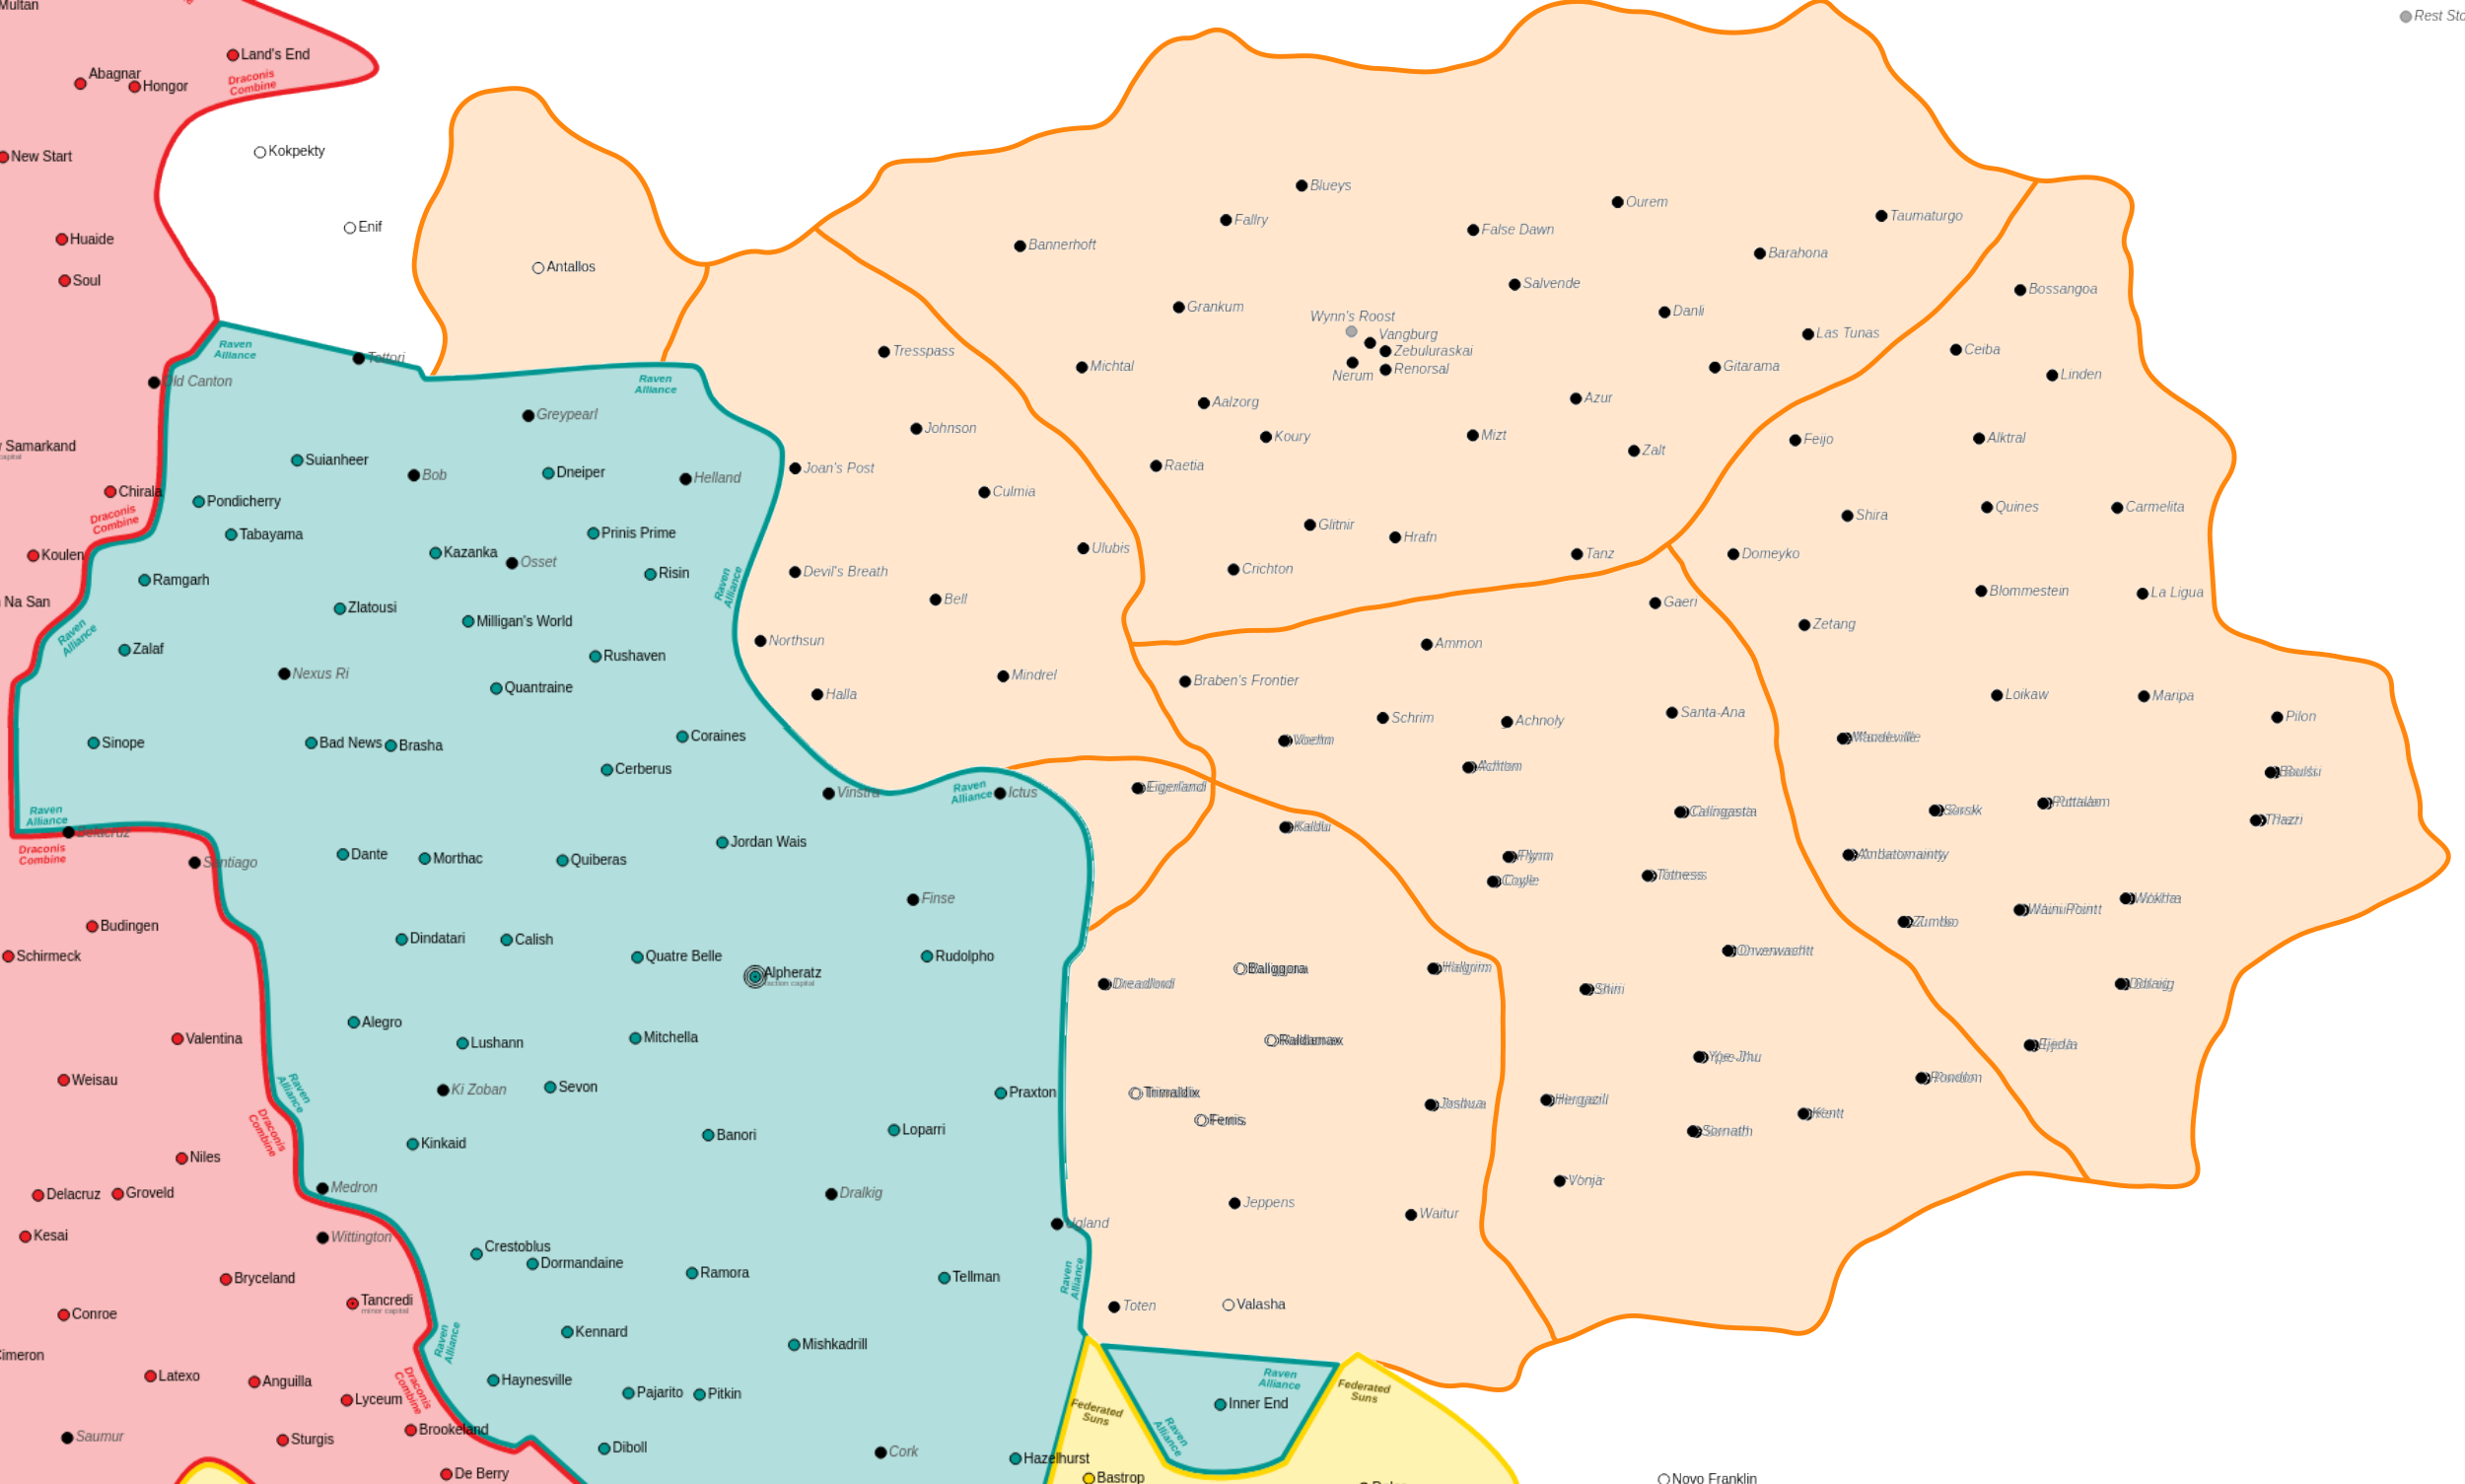
\includegraphics[width=8.9in,keepaspectratio]{../img/Outworlds_Wastes_ilClan_Map.png}}
  \rotatebox{90}{%
    \begin{minipage}{\wd\savefig}
      \usebox{\savefig}
      \caption*{Outworlds Wastes - 3151}
    \end{minipage}}
\end{figure}

\newpage

% --------------------------------------------------------------------------------
% --------------------------------------------------------------------------------
\section{Sample Force Roster}
% --------------------------------------------------------------------------------
% --------------------------------------------------------------------------------

\begin{table}[h!]
\fontfamily{Montserrat-LF}\selectfont
\centering
\newcolumntype{R}[1]{>{\raggedleft\let\newline\\\arraybackslash\hspace{0pt}}m{#1}}
\begin{tabular}{| m{1.5em} m{11em} m{8em} R{4.7em} R{4.5em} R{3.5em} R{3.5em} |}
\hline
\rowcolor{black!30} \bfseries{Bay} & \bfseries{Unit} & \bfseries{Pilot} & \bfseries{Gunnery} & \bfseries{Piloting} & \bfseries{C-bills} & \bfseries{BV} \\
\hline
\rowcolor{black!30} \multicolumn{7}{|c|}{Mechs (1 per bay)} \\
\hline
1  & & & & & & \\
2  & & & & & & \\
3  & & & & & & \\
4  & & & & & & \\
5  & & & & & & \\
6  & & & & & & \\
7  & & & & & & \\
8  & & & & & & \\
9  & & & & & & \\
10 & & & & & & \\
11 & & & & & & \\
12 & & & & & & \\
\hline
\rowcolor{black!30} \multicolumn{7}{|c|}{Combat Vehicles (2 per bay)} \\
\hline
1 & & & & & & \\
1 & & & & & & \\
2 & & & & & & \\
2 & & & & & & \\
3 & & & & & & \\
3 & & & & & & \\
4 & & & & & & \\
4 & & & & & & \\
5 & & & & & & \\
5 & & & & & & \\
\hline
\rowcolor{black!30} \multicolumn{7}{|c|}{Aerospace (2 per bay)} \\
\hline
1 & & & & & & \\
1 & & & & & & \\
2 & & & & & & \\
2 & & & & & & \\
\hline
\rowcolor{black!30} \multicolumn{7}{|c|}{Protomechs (5 per bay)} \\
\hline
1 & & & & & & \\
1 & & & & & & \\
1 & & & & & & \\
1 & & & & & & \\
1 & & & & & & \\
2 & & & & & & \\
2 & & & & & & \\
2 & & & & & & \\
2 & & & & & & \\
2 & & & & & & \\
\hline
\rowcolor{black!30} \multicolumn{7}{|c|}{Infantry/Battle Armor (5 tons per bay)} \\
\hline
1  & & & & & & \\
2  & & & & & & \\
3  & & & & & & \\
4  & & & & & & \\
5  & & & & & & \\
\hline
  & Total Bays (16 max) & & & & & \\
  & Total BV   & & & & & \\
\hline
\end{tabular}
\end{table}

\newpage

% --------------------------------------------------------------------------------
% --------------------------------------------------------------------------------
\section{Sample Scenario Logistics Tracking}
% --------------------------------------------------------------------------------
% --------------------------------------------------------------------------------

\begin{table}[h!]
\fontfamily{Montserrat-LF}\selectfont
\centering
\newcolumntype{R}[1]{>{\raggedleft\let\newline\\\arraybackslash\hspace{0pt}}m{#1}}
\begin{tabular}{| m{27em} R{15em} |}
\hline
\rowcolor{black!30} \bfseries{Item} & \bfseries{C-bills} \\
\hline
\rowcolor{black!30} \multicolumn{2}{|c|}{Starting Balance} \\
\hline
 & \\
\hline
\rowcolor{black!30} \multicolumn{2}{|c|}{Objectives} \\
\hline
Primary Objective               & \\
Secondary Objective             & \\
Base Pay (if no objectives met) & \\
\hline
\rowcolor{black!30} \multicolumn{2}{|c|}{Training} \\
\rowcolor{black!30} \multicolumn{2}{|c|}{Pay 500,000 $\times$ BV skill multiplier difference} \\
\hline
1 & \\
2 & \\
3 & \\
4 & \\
5 & \\
... & \\
\hline
\rowcolor{black!30} \multicolumn{2}{|c|}{Maintenance (Replace, Repair, and Recruit)} \\
\rowcolor{black!30} \multicolumn{2}{|c|}{Pay 50\% cost if destroyed, 25\% cost to repair internal damage} \\
\rowcolor{black!30} \multicolumn{2}{|c|}{Pay 50\% cost per troop killed} \\
\hline
1 & \\
2 & \\
3 & \\
4 & \\
5 & \\
... & \\
\hline
\rowcolor{black!30} \multicolumn{2}{|c|}{Refits} \\
\rowcolor{black!30} \multicolumn{2}{|c|}{Pay cost difference to change variants} \\
\hline
1 & \\
2 & \\
3 & \\
4 & \\
5 & \\
... & \\
\hline
\rowcolor{black!30} \multicolumn{2}{|c|}{Purchases} \\
\rowcolor{black!30} \multicolumn{2}{|c|}{Pay cost to add to TOE} \\
\hline
1 & \\
2 & \\
3 & \\
... & \\
\hline
\rowcolor{black!30} \multicolumn{2}{|c|}{Salvage} \\
\rowcolor{black!30} \multicolumn{2}{|c|}{Pay 50\% cost to add to TOE or sell to earn 25\% cost} \\
\hline
1 & \\
2 & \\
3 & \\
... & \\
\hline
\rowcolor{black!30} \multicolumn{2}{|c|}{Total} \\
\hline
 & \\
\hline
\end{tabular}
\end{table}

\newpage

% --------------------------------------------------------------------------------
% --------------------------------------------------------------------------------
\section{Force BV Adjustments}
\label{sec:force_bv_adjustments}
% --------------------------------------------------------------------------------
% --------------------------------------------------------------------------------

\begin{table}[h!]
\fontfamily{Montserrat-LF}\selectfont
\centering
\newcolumntype{C}[1]{>{\centering\let\newline\\\arraybackslash\hspace{0pt}}m{#1}}
\begin{tabular}{| C{4.7em} | C{3em} C{3em} C{3em} C{3em} C{3em} C{3em} C{3em} C{3em} |}
\hline
\rowcolor{black!30} \bfseries{Gunnery} & \multicolumn{8}{c |}{\bfseries{Piloting/Driving/Anti-Mech}}  \\
\hline
  & 1    & 2    & 3    & 4    & 5    & 6    & 7    & 8    \\
\hline
1 & 2.11 & 2.02 & 1.92 & 1.76 & 1.60 & 1.54 & 1.46 & 1.38 \\
2 & 1.85 & 1.76 & 1.68 & 1.54 & 1.40 & 1.35 & 1.28 & 1.21 \\
3 & 1.58 & 1.51 & 1.44 & 1.32 & 1.20 & 1.16 & 1.10 & 1.04 \\
4 & 1.32 & 1.26 & 1.20 & 1.10 & 1.00 & 0.95 & 0.90 & 0.85 \\
5 & 1.19 & 1.13 & 1.08 & 0.99 & 0.90 & 0.86 & 0.81 & 0.77 \\
6 & 1.12 & 1.07 & 1.02 & 0.94 & 0.85 & 0.81 & 0.77 & 0.72 \\
7 & 1.06 & 1.01 & 0.96 & 0.88 & 0.80 & 0.76 & 0.72 & 0.68 \\
8 & 0.99 & 0.95 & 0.90 & 0.83 & 0.75 & 0.71 & 0.68 & 0.64 \\
\hline
\end{tabular}
\end{table}

\begin{itemize}

\item Each unit equipped with TAG or a C\textsuperscript{3} master computer adds BV for each  ton of semi-guided LRM ammunition carried by all units in the force.

\item Each unit that is part of a C\textsuperscript{3} network increases its BV by 5\% of the total BV of all units included in the C\textsuperscript{3} network.

\end{itemize}

This summary is provided here for convenience.
\emph{BattleTech: TechManual} page 315 and any relevant errata supersedes this information.

\newpage

% --------------------------------------------------------------------------------
% --------------------------------------------------------------------------------
\section{References}
% --------------------------------------------------------------------------------
% --------------------------------------------------------------------------------

The following references are mentioned in these rules

\begin{itemize}

\item \emph{BattleTech: Total Warfare}

\item \emph{BattleTech: BattleMech Manual}

\item \emph{BattleTech: TechManual}

\item \emph{BattleTech: Tactical Operations Advanced Rules}

\item \emph{BattleTech: Tactical Operations Advanced Units \& Equipment}

\item \emph{BattleTech: Campaign Operations}

\item \emph{Alpha Strike: Commander's Edition}

\item \emph{Master Unit List}: \href{http://www.masterunitlist.info}{http://www.masterunitlist.info}

\item \emph{MegaMek}: \href{https://megamek.org}{https://megamek.org}

\item \emph{Sarna.net}: \href{https://sarna.net}{https://sarna.net}

\item \emph{Death From Above Wargaming}: \href{https://dfawargaming.com}{https://dfawargaming.com}

\end{itemize}

\newpage

% --------------------------------------------------------------------------------
% --------------------------------------------------------------------------------
% End page
% --------------------------------------------------------------------------------
% --------------------------------------------------------------------------------

\clearpage

\title{
  \fontfamily{Montserrat-TOsF}\selectfont
  \fontsize{50}{60}\fontseries{ub}\selectfont\textcolor{white}{\MakeUppercase{B}}
\includegraphics[width=0.5in]{../img/Battletech_A.png}\fontsize{50}{60}\fontseries{ub}\selectfont\textcolor{white}{\MakeUppercase{ttleTech}}\\
  \fontsize{35}{42}\fontseries{ub}\selectfont\MakeUppercase{Outworlds Wastes}
}

% --------------------------------------------------------------------------------
\maketitle
% --------------------------------------------------------------------------------

\AddToHookNext{shipout/background}
{\put(0,-\paperheight)
  {%
   
\begin{tikzpicture}
   \fill[use as bounding box,black!10] (current page.north west) rectangle (\paperwidth,0);
   \fill[use as bounding box,black!50] ($ (current page.north west)+(0,-12.3) $) rectangle ++(\paperwidth,-1.7);
   \fill[use as bounding box,black!30] ($ (current page.north west)+(0,-14.0) $) rectangle ++(\paperwidth,-1.6);
   \end{tikzpicture}
  }
}

\thispagestyle{empty}

\end{document}
% --------------------------------------------------------------------------------
